\documentclass[11pt]{article}
\ifdefined\pdftrailerid\pdftrailerid{}\fi
\ifdefined\pdfinfoomitdate\pdfinfoomitdate=1\fi
\usepackage[T1]{fontenc}
\usepackage{lmodern,amsmath,amssymb,amsthm,mathtools,microtype,booktabs}
\ifdefined\pdfglyphtounicode
  \pdfgentounicode=1
  \pdfglyphtounicode{tfm:lmex10/parenleftbig}{0028}
  \pdfglyphtounicode{tfm:lmex10/parenrightbig}{0029}
  \pdfglyphtounicode{tfm:lmex10/parenleftbigg}{0028}
  \pdfglyphtounicode{tfm:lmex10/parenrightbigg}{0029}
  \pdfglyphtounicode{tfm:lmex10/integraltext}{222B}
  \pdfglyphtounicode{tfm:lmex10/integraldisplay}{222B}
  \pdfglyphtounicode{tfm:lmex10/summationdisplay}{2211}
  \pdfglyphtounicode{tfm:lmex10/hatwide}{02C6}
  \pdfglyphtounicode{tfm:lmex10/bracelefttp}{23A7}
  \pdfglyphtounicode{tfm:lmex10/braceleftmid}{23A8}
  \pdfglyphtounicode{tfm:lmex10/braceleftbt}{23A9}
  \pdfglyphtounicode{tfm:lmex10/braceex}{23AA}
  \pdfglyphtounicode{tfm:lmsy10/mapsto}{007C}
  \pdfglyphtounicode{tfm:lmsy10/L}{2112}
  \pdfglyphtounicode{tfm:lmsy10/O}{1D4AA}
  \pdfglyphtounicode{tfm:lmsy10/T}{1D4AF}
  \pdfglyphtounicode{tfm:msbm10/R}{211D}
  \pdfglyphtounicode{tfm:msbm10/T}{1D54B}
  \pdfglyphtounicode{tfm:msbm10/Z}{2124}
  \pdfglyphtounicode{tfm:lmmi10/mu}{03BC}
  \pdfglyphtounicode{tfm:lmmi8/mu}{03BC}
  \pdfglyphtounicode{tfm:rm-lmr10/Delta}{0394}
  \pdfglyphtounicode{tfm:rm-lmbx10/d}{1D41D}
  \pdfglyphtounicode{tfm:rm-lmbx10/h}{1D421}
  \pdfglyphtounicode{tfm:rm-lmbx10/u}{1D42E}
  \pdfglyphtounicode{tfm:rm-lmbx10/w}{1D430}
  \pdfglyphtounicode{tfm:lmmib10/pi}{1D745}
  \pdfglyphtounicode{tfm:rm-lmss8/T}{1D5B3}
\fi
\usepackage[margin=1in]{geometry}
\usepackage{xcolor,tikz,needspace}
\usetikzlibrary{arrows.meta,positioning}
\usepackage[colorlinks=true,linkcolor=blue!50!black,citecolor=blue!50!black,urlcolor=blue!50!black]{hyperref}
\hypersetup{pdftitle={Universal Computation with Eventually Stationary Navier--Stokes Forcing},pdfauthor={OpenAI}}
\newtheorem{theorem}{Theorem}[section]
\newtheorem{lemma}[theorem]{Lemma}
\newtheorem{proposition}[theorem]{Proposition}
\newtheorem{corollary}[theorem]{Corollary}
\theoremstyle{remark}\newtheorem{remark}[theorem]{Remark}
\newcommand{\T}{\mathbb T}\newcommand{\R}{\mathbb R}
\newcommand{\Z}{\mathbb Z}\newcommand{\N}{\mathbb N}
\DeclareMathOperator{\diver}{div}
\DeclareMathOperator{\supp}{supp}
\title{Universal Computation with Eventually Stationary Navier--Stokes Forcing}
\author{OpenAI}
\date{September 27, 2026}
\begin{document}\maketitle
\begin{abstract}
At every fixed positive computable viscosity, we construct smooth
mean-zero forces on the flat three-torus that become stationary after
time one and make a fixed particle, initially in a fluid at rest, enter
a fixed open set exactly when a prescribed Turing machine halts.
The force has bounded derivatives of every order and a finite effective
description. A reversible recording table is realized on whole planar
rectangles by Hamiltonian motions, then driven by a mean-zero spatial
clock. Separate choices give periodic forcing from time zero or a
force whose derivatives are square-integrable in time.
\end{abstract}

\section{Introduction and result}\label{sec:introduction}
Can a force that eventually stops changing continue to perform an
arbitrarily long computation? We ask this for the incompressible
Navier--Stokes equation with a fixed flat geometry, fixed viscosity and
zero initial velocity. The observation is equally fixed: one material
particle must enter a specified open region. Only the finite prescription
of the force may depend on the machine and its input.

An exact real coordinate can retain an unbounded tape as a positional
expansion. Moore's generalized shifts convert local tape instructions
into piecewise affine maps and relate their smooth realizations to
three-dimensional flows \cite{Moore1990,Moore1991}. A difficulty is that
a tape instruction may erase information whereas a smooth flow has
invertible finite-time maps. Landauer discusses retaining intermediate
information to avoid this loss \cite[Section~3]{Landauer1961}; Bennett
implements reversible simulation by recording instruction indices
\cite[Eqs.~(9)--(11)]{Bennett1973}. Our finite recording table follows
that information-retention principle. Its seven rows and full-domain
inverse are proved here, rather than imported from a reversible-machine
existence theorem.

Fluid versions of computational universality already exist in different
geometric settings. Cardona, Miranda, Peralta-Salas and Presas obtain
stationary Euler flows on an adapted Riemannian three-sphere, using an
area-preserving realization of generalized shifts and a suspension
\cite{CardonaMirandaPeraltaSalasPresas2021}. Dyhr, Gonz\'alez-Prieto, Miranda and Peralta-Salas
obtain stationary unforced Navier--Stokes universality using an adapted
metric and the Hodge Laplacian \cite{DyhrGonzalezPrietoMirandaPeraltaSalas2026}. The geometric ancestry includes the Reeb--Beltrami correspondence
of Etnyre and Ghrist \cite{EtnyreGhrist2000} and the earlier
higher-dimensional Euler realization in
\cite{CardonaMirandaPeraltaSalasPresas2023}, first posted in 2019.
These Euler and Hodge-viscous constructions choose the geometry and
use stationary initial velocity. Here the flat metric is fixed and the
fluid starts at rest. We place the machine in an external force and
prove its construction directly.

Fixed-metric Euler computation also has
important precedents: Cardona, Miranda and Peralta-Salas construct an
unrestricted steady Euler simulation on Euclidean $\R^3$ with infinite
energy \cite[arXiv version~3, Theorem~1]{CardonaMirandaPeraltaSalas2023Beltrami}.
They also give a robust tape-bounded simulation on the flat three-torus,
with observation restricted to the initial trajectory segment before
exit from a specified compact region
\cite[arXiv version~3, Theorem~26]{CardonaMirandaPeraltaSalas2023Beltrami}.
Their Remark~29 gives an unforced viscous tape-bounded version with
nonzero Beltrami initial velocity. The compact forced viscous experiment
here starts from rest and permits an unbounded computation.

The force identity itself is elementary: for a prescribed incompressible
velocity, its material acceleration minus its viscous term is a body
force. The substance of the argument is to prescribe the velocity from
the finite machine table without running that machine. We first retain
the history needed for an inverse. Gapped tape coordinates then give
separated source rectangles and, independently, separated target
rectangles. The two families may overlap. Ordered extraction to a
parking region, reciprocal deformation and ordered delivery realize
every branch by an area-preserving motion. A third spatial coordinate
supplies the phase. A fixed ramp starts this autonomous field from rest,
after which the force is stationary.

Write $\T=\R/\Z$ and $x=(X,Y,Z)\in\T^3$. We use
\begin{equation}\label{eq:NS}
 \partial_tu+(u\cdot\nabla)u=-\nabla p+\nu\Delta u+f,
 \qquad \diver u=0,\qquad u(0)=0.
\end{equation}
The Laplacian is the componentwise flat Laplacian and pressure has mean
zero. A classical solution has continuous $u$, $u_t$, spatial derivatives
of $u$ through order two, $p$ and $\nabla p$ on every closed finite
time cylinder. All constructed solutions are smooth. For a particle
label $a$, the material trajectory solves
$\dot\Phi(t,a)=u(t,\Phi(t,a))$, $\Phi(0,a)=a$.

An effective smooth force is supplied by a finite program that evaluates
every requested mixed derivative at computably supplied space-time
arguments to any prescribed rational error. It also computes the
derivative bounds used below. There is no efficiency requirement, but
the program must describe all branches of the mechanism; it cannot
first compute the selected execution and replay it.

\begin{theorem}[Eventually steady forcing]\label{thm:main}
Fix a positive computable viscosity $\nu$.  There is an effective
procedure taking a deterministic Turing machine and finite input to
a body force $f$ on the flat torus $\mathbb T^3$, such that:
\begin{enumerate}
\item $f$ is smooth on $\mathbb T^3\times[0,\infty)$, has zero
spatial mean, and is independent of time for $t\ge1$.  Every spatial,
temporal, and mixed derivative of $f$ is bounded on this entire domain.
\item With initial velocity zero, the Navier--Stokes equation has a
global smooth solution, unique in the classical class on every finite
time interval.  Its kinetic energy is bounded uniformly in time.
\item For the fixed particle label and fixed open set
\[
 P=(1/4,1/4,0),\qquad
 \mathcal O=\{(X,Y,Z)\in\mathbb T^3:1/32<Y<1/8\},
\]
the material trajectory from $P$ enters $\mathcal O$ at a finite
time if and only if the machine halts on the input.
\end{enumerate}
The force is specified by a finite formula which does not simulate the
chosen execution.  The construction is also uniform as a formula in
an arbitrary positive parameter $\nu$.
\end{theorem}
For a fixed positive noncomputable $\nu$, the same finite formulas and
mathematical conclusions hold, with evaluation relative to that
parameter. The algorithmic assertion concerns computable $\nu$.
The force can also be made solenoidal by the periodic
Helmholtz--Leray projection; this changes the pressure, not the velocity.
Theorem~\ref{thm:main} concerns these explicitly supplied smooth
solutions and is not a regularity theorem for arbitrary fluid data.

The undecidability is about exact trajectories; the theorem supplies no
uniform finite-precision tolerance for the infinite encoded computation.
Finite-time perturbation bounds will nevertheless be quantitative and
effective. They also permit the planar construction to be used in
diffusion problems where control of small neighborhoods is essential.

Section~\ref{sec:analytic} gives the short analytic tools. Section~\ref{sec:compiler}
constructs the recording table and proves its inverse and initialization.
Section~\ref{sec:processor} gives the complete planar geometry and its
derivative bounds. Section~\ref{sec:lagrangian} supplies the spatial
clock and proves Theorem~\ref{thm:main}. Section~\ref{sec:profiles}
gives the slow temporal alternative. The periodic alternative is obtained
directly from the planar field and therefore requires no loading interval.

\section{Effective profiles and analytic realization}\label{sec:analytic}
We will construct a smooth velocity explicitly. The three lemmas in this
section explain how its finite formulas can be evaluated at cutoff
endpoints and how its residual determines a unique fluid solution.

\begin{lemma}[Flat profiles]\label{lem:profiles}
Put $E(t)=e^{-1/t}$ for $t>0$ and $E(t)=0$ for $t\le0$, and put
$\beta(t)=E(t)/(E(t)+E(1-t))$. These functions are computably smooth.
The function $\beta$ is zero for $t\le0$, one for $t\ge1$, and satisfies
$\beta(t)+\beta(1-t)=1$. Products of rational translates and rescalings
give effective cutoffs equal to one near a prescribed rational closed
box and supported in any prescribed larger open rational box.
All their derivatives have effective bounds.
\end{lemma}
\begin{proof}
On $t>0$ the $j$th derivative of $E$ is
$P_j(1/t)e^{-1/t}$, where the polynomial $P_j$ is generated recursively.
For integers $m,k\ge0$ and $y>0$,
$y^m e^{-y}\le(m+k)!y^{-k}$. These estimates prove flatness and give
an effective error tending to zero as $t\downarrow0$. Away from zero,
ordinary arithmetic and the exponential evaluate the derivatives.
The denominator defining $\beta$ is at least $e^{-2}$, since at least
one of $t,1-t$ is at least $1/2$. Quotient differentiation is therefore
effective even when equality with an endpoint is undecidable.
For $a<b<c<d$ the product
$\beta((t-a)/(b-a))\beta((d-t)/(d-c))$ has the required interval
plateau; coordinate products give boxes. The derivative bounds follow
by the product and chain rules and the preceding estimates.

For later periodic evaluation, let $F_0$ be a smooth function on $[0,1]$
that is zero near the endpoints, extended by zero to $\R$.
Given a computably supplied $s\in\R$, compute a rational $q$ with
$|q-s|<1$. Its periodization and all derivatives are finite sums:
\[
 F_{\rm per}^{(j)}(s)=
 \sum_{k=\lfloor q\rfloor-2}^{\lceil q\rceil+2}F_0^{(j)}(s-k).
\]
Every omitted translate is zero, since a nonzero term requires
$k\in[s-1,s]$. Floors and ceilings are taken only of the rational $q$,
so no integer-part test is made on $s$. The same coordinatewise finite
sum evaluates spatial periodizations of compact chart-supported fields.
This supplies the finite-index bound for the periodic pulses below.
\end{proof}

\begin{lemma}[Prescribed velocity and comparison]\label{lem:realization}
Let $U$ be a smooth divergence-free velocity on
$[0,\infty)\times\T^3$ with $U(0)=0$. Define
\begin{equation}\label{eq:residual}
 F=U_t+(U\cdot\nabla)U-\nu\Delta U.
\end{equation}
Then $(U,0)$ is a global smooth solution of \eqref{eq:NS} with force
$F$, unique in the classical class on every finite time interval.
If $U$ has zero spatial mean, so does $F$.
\end{lemma}
\begin{proof}
Substitution proves existence. To prove uniqueness, use the classical
difference-energy method \cite[Section~18]{Leray1934}. For another
solution $(v,p)$ with the same force and data set $w=v-U$.
Its equation is
\[
 w_t+(v\cdot\nabla)w+(w\cdot\nabla)U-\nu\Delta w+\nabla p=0.
\]
The stated regularity permits multiplication by $w$ and periodic
integration by parts. The pressure and transport terms vanish, giving
\[
 \frac12\frac{d}{dt}\|w\|_2^2+\nu\|\nabla w\|_2^2
 \le\|\nabla U\|_{\infty,\mathrm{op}}\|w\|_2^2.
\]
On every finite interval the coefficient is bounded. Gronwall's
inequality and $w(0)=0$ give $w=0$; the pressure gradient then vanishes,
and its normalization gives $p=0$. Smoothness on compact time cylinders
also gives a unique material flow through every finite time.
Finally, each component of $(U\cdot\nabla)U$ is the divergence of a
periodic vector field, and the integral of $\Delta U$ vanishes.
Integrating \eqref{eq:residual} proves the mean assertion.
\end{proof}

\begin{lemma}[Solenoidal projection]\label{lem:projection}
A computably smooth mean-zero force $F$ on $\T^3$, with effective
spatial derivative bounds, can be replaced by a computably smooth
mean-zero solenoidal force $F-\nabla\phi$, where
$\Delta\phi=\diver F$ and $\int\phi=0$. Replace the pressure $p$
by $p-\phi$. The velocity is unchanged. Eventual stationarity,
periodicity and bounds for mixed derivatives are preserved. Any
temporal $L^2$ estimates for all spatial derivative orders are preserved
as well.
\end{lemma}
\begin{proof}
In the Fourier basis $e^{2\pi i k\cdot x}$ set
\[
 \widehat\phi(k)=-\frac{i k\cdot\widehat F(k)}{2\pi|k|^2}
 \quad(k\ne0),\qquad \widehat\phi(0)=0.
\]
The multiplier for $\nabla\phi$ is $kk^{\mathsf T}/|k|^2$ and has
operator norm one. For a derivative order $r$, integrate the coefficient
of $F$ by parts $r+5$ times in a coordinate with largest $|k_i|$.
There are at most $C n^2$ lattice points with $n\le|k|<n+1$, so the
derivative series converges absolutely with a computable tail, and
\[
 \|\partial_t^h\partial_x^\mu\nabla\phi(t)\|_\infty
 \le C_\mu\max_i
 \|\partial_t^h\partial_{x_i}^{|\mu|+5}F(t)\|_\infty.
\]
This proves the asserted uniform and temporal bounds. Riemann sums
with derivative error bounds evaluate each Fourier coefficient; the
series tail makes the resulting procedure effective. Differentiation
in time commutes with this fixed spatial multiplier. Substitution gives
$-\nabla(p-\phi)+(F-\nabla\phi)=-\nabla p+F$, which checks the
pressure sign and completes the proof.
\end{proof}

\section{A finite reversible rule table}\label{sec:compiler}

We use deterministic machines with one head on a tape indexed by
$\mathbb Z$, a finite alphabet containing a blank, and head moves in
$\{-1,0,1\}$.  The finite input occupies cells $0,\ldots,r-1$, all
other cells are blank, and the head starts at $0$.  A transition writes
one symbol before moving the head.  A machine can effectively be put
in the convention of a single halting state $q_{\rm H}$, no rules
there, and a total table elsewhere: missing instructions and multiple
halting states can be redirected to a new halting state.  We also add
a fresh initial state $q_{\rm start}$ whose rules leave the symbol and
head unchanged and enter the former initial state.  This extra step
preserves halting, even when the original initial state was halting.

Fluid maps are invertible.  We therefore first retain the information
that a machine transition would otherwise erase.  History recording
is the classical way to obtain reversible computation
\cite[Eqs.~(9)--(11)]{Bennett1973}; the following explicit version also has the local
property needed for our geometric construction.

\begin{lemma}[An injective local compiler]\label{lem:compiler}
From a deterministic machine and its finite input one can effectively
construct a finite partial one-head transition table and an initial
tape which differs from a constant blank tape at finitely many cells,
with these properties.
\begin{enumerate}
\item Its initialized run reaches a single terminal state, which has
no outgoing rules, if and only if the original machine halts.  Otherwise
every successive transition is defined and the run continues forever.
At specified finite checkpoints its state and tape recover the original
computation.
\item All rules arriving at a fixed state have the same head displacement.
The destination state and the full written symbol determine the incoming
rule, including its old state and read symbol.
\end{enumerate}
\end{lemma}

\begin{proof}
Let $Q$ and $\Gamma$ be the states and alphabet of the augmented machine.
For each $\tau=(q,a)$ in
$\mathcal T=(Q\setminus\{q_{\rm H}\})\times\Gamma$, write its
instruction as $(q_\tau^+,a_\tau^+,d_\tau)$.  Use the three-track alphabet
\[
 \Sigma=\Gamma\times\{0,1\}\times\mathcal L,
 \qquad \mathcal L=\{\bot,E\}\sqcup\mathcal T.
\]
The tracks hold data, a head marker, and history, respectively.  The
states are $R_q,C_q,L_q$ for $q\in Q$ and $A_\tau,F_\tau$ for
$\tau\in\mathcal T$, all distinguished by their types and subscripts.
Only $R_{q_{\rm H}}$ is terminal.  Initially the state is
$R_{q_{\rm start}}$, the data and head are the given data and head, all
marker bits vanish, and the history is $E$ at cell $2$ and $\bot$
elsewhere.  Thus the full blank symbol is $(\text{blank},0,\bot)$.

The intended invariant at the ready checkpoint after $n$ augmented
steps is the following: the control is $R_q$, and its data and head $h$
are exactly those of the augmented machine, with $|h|\le n$. Every
marker bit vanishes. History cells $2,\ldots,n+1$ contain the successive
$n$ instruction tags, cell $n+2$ contains $E$, and every other history
cell contains $\bot$. We prove this invariant below.

The next transition first performs the data instruction and enters
$A_\tau$. It then marks the new head position and enters the forward
scan $F_\tau$. That scan reaches $E$, replaces it by the instruction
record $\tau$, and enters $C_{q_\tau^+}$ one cell to its right.
The $C$ step advances the frontier to that empty cell and turns into
$L_{q_\tau^+}$. The leftward scan returns to the marked work-head
position, erases the mark, and enters the next ready state. The
frontier always lies beyond the new work head; the temporary marker
remembers where the returning scan must stop.

Here is the entire partial table.  Each row is expanded over all
symbols satisfying its displayed restrictions; $a\in\Gamma$ and
$\ell\in\mathcal L$.
\begin{equation}\label{eq:compiler-table}
\begin{array}{lll}
(R_q,(a,0,\ell)) &\longmapsto
 (A_\tau,(a_\tau^+,0,\ell),d_\tau)
 &q\ne q_{\rm H},\ \tau=(q,a),\ \ell\ne E,\\
(A_\tau,(a,0,\ell)) &\longmapsto
 (F_\tau,(a,1,\ell),1)&\ell\ne E,\\
(F_\tau,(a,0,\ell)) &\longmapsto
 (F_\tau,(a,0,\ell),1)&\ell\ne E,\\
(F_\tau,(a,0,E)) &\longmapsto
 (C_{q_\tau^+},(a,0,\tau),1),&\\
(C_q,(a,0,\bot)) &\longmapsto
 (L_q,(a,0,E),-1),&\\
(L_q,(a,0,\ell)) &\longmapsto
 (L_q,(a,0,\ell),-1)&\ell\ne E,\\
(L_q,(a,1,\ell)) &\longmapsto
 (R_q,(a,0,\ell),0)&\ell\ne E.
\end{array}
\end{equation}

The invariant holds initially. To verify its induction step, the first row performs
the data instruction and moves to $h'=h+d_\tau\le n+1<n+2$.
The second row marks $h'$ and starts a rightward scan.  The third and
fourth rows reach the finite frontier $n+2$, replace $E$ by $\tau$,
and advance one cell.  The fifth row writes the new frontier at $n+3$
and turns left.  The last two rows return to the unique marker, erase
it, and enter $R_{q_\tau^+}$ at $h'$.  This takes
$4+2(n+2-h')$ transitions, a positive finite number.  No undefined
rule is encountered.  Halting and the checkpoint correspondence follow.

For completeness, the local injectivity can be checked destination by
destination.  Into $A_\tau$, the tag fixes the old state and data
symbol, and the written symbol retains the old history letter.  Into
$F_\tau$ both incoming types move right; the arrival from $A_\tau$
writes marker $1$, whereas the scan loop writes marker $0$.  Into
$C_q$ the move is right and the written tag identifies $\tau$, while
the data letter is retained.  Into $L_q$ both types move left; the
arrival from $C_q$ writes $E$, whereas the loop never does.  Into
$R_q$ only the last row applies, with displacement zero and the data
and history letters retained.  In every case the destination and
written full symbol recover the unique expanded rule.
In particular the full configuration map is injective on its domain:
from a destination configuration its state fixes $d$, so the old head
was at the new head minus $d$; the symbol at that cell identifies the
rule and hence the old read symbol and state.  Restoring that one
symbol recovers the entire predecessor configuration.
\end{proof}

\section{An area-preserving planar processor}\label{sec:processor}

The next construction realizes the entire finite rule table in one
period. Area-preserving realization of generalized shifts is also a
central step in \cite[Proposition~5.1]{CardonaMirandaPeraltaSalasPresas2021}.
Here we give explicit local Hamiltonian motions, quantitative flow bounds
and a corridor respected at every intermediate time.  In particular, it does not construct the sequence of branches
visited by the chosen input.

\begin{theorem}[A smooth planar processor]\label{thm:planar-processor}
From the machine and input one can effectively construct a smooth
field $V(s,X,Y)$ on $\mathbb R\times\mathbb T^2$ with the following
properties.
\begin{enumerate}
\item $V$ is $1$-periodic in $s$, vanishes on neighborhoods of integer
$s$, is divergence free in $(X,Y)$, and has zero spatial mean.
Its planar support is a compact subset of the open unit-square chart.
It has a smooth periodic Hamiltonian potential supported in that chart.
The same formula, extended by zero, defines a compactly supported field
on $\R^2$ with the same conclusions below. The construction also
supplies a finite list of closed rational source rectangles $D_r$, target
rectangles $H_r$ and affine maps $F_r:D_r\to H_r$, each with positive
reciprocal diagonal linear part. The two rectangle families are
separately disjoint. These maps implement the symbolic branches under
an explicit tape encoding. The period map agrees with $F_r$ on a
positive neighborhood of $D_r$, with an effective lower bound for
the neighborhood radius.
All its derivatives have effective finite uniform bounds.
\item Starting from $p=(1/4,1/4)$ at $s=0$, the trajectory at successive
integer times encodes every transition of the compiled machine, until
its terminal state is reached.  All these trajectory segments lie in
\[
 J_*=[1/8,7/8]\times[1/32,7/8].
\]
The trajectory reaches the fixed strip
\[
 H=\{(X,Y)\in\mathbb T^2:1/32<Y<1/8\}
\]
at a finite time if and only if the original machine halts.  If the
machine does not halt, $3/16\le Y\le7/8$ throughout the trajectory.
If it halts, an integer-time point lies in $H$ at distance at least
$1/32$ from its boundary.
\item One can compute $L\ge1$ such that planar transition maps over
any phase interval of length $s\ge0$, and their inverses, have first
derivative norm at most $e^{Ls}$ and second derivative norm at most
$e^{2Ls}-e^{Ls}$. Here $L$ bounds both $D_{X,Y}V$ and
$D_{X,Y}^2V$ globally. Perturbations of an initial point are magnified by at most
$e^{Ls}$ over such an interval.
\end{enumerate}
\end{theorem}

\subsection{Separated radix coordinates}

The passage from symbolic rules to affine maps is the generalized-shift
construction of Moore~\cite{Moore1990,Moore1991}. We specify the gapped coordinates and
verify the full rectangle maps needed for smooth incompressible motion.

Write $K=|\Sigma|$, put $B=2K+2$, and assign the symbols distinct odd
digits $c(a)\in\{1,3,\ldots,2K-1\}$.  Define
\[
 C(a_1,a_2,\ldots)=\sum_{k\ge1}\frac{c(a_k)}{B^k},
 \qquad I_a=\frac{c(a)+[0,1]}B,
 \qquad I_{a,b}=\frac{c(a)+I_b}B.
\]
Every sequence code lies in
$[1/(B-1),(2K-1)/(B-1)]\subset(0,1)$.  The closed intervals
$I_a$ are separated by positive gaps, as are the intervals $I_{a,b}$
for distinct ordered pairs.  A sequence code lies in the interior of
its first-symbol interval.  Reading that interval and rescaling
recovers the tail, so the sequence representation is unique.

For a compiled configuration with state $i$, head $h$, and tape
$(a_k)_{k\in\mathbb Z}$, use head-relative coordinates
\begin{equation}\label{eq:two-stack-code}
 x=C(a_{h-1},a_{h-2},\ldots),\qquad
 y=C(a_h,a_{h+1},\ldots).
\end{equation}
The initial coordinates $x_0,y_0$ are computable rationals: the finite
nonblank part is followed on each side by a geometric constant-symbol
tail.  Let $m$ be the number of compiled states and let $N$ be the number
of branches obtained by counting a displacement $0$ or $1$ rule once,
and a displacement $-1$ rule $K$ times.  There is at least one rule.
Set
\[
 \lambda=\frac1{100(m+N+1)},\qquad a_* =\frac14-\lambda x_0.
\]
Associate to each state a square using
\begin{equation}\label{eq:state-squares}
 \Psi_i(x,y)=(a_*+\lambda x,b_i+\lambda y),\qquad
 b_i=
 \begin{cases}
  1/4-\lambda y_0,&i=R_{q_{\rm start}},\\
  1/16,&i=R_{q_{\rm H}},\\
  1/3+\ell/[12(m+1)],&i\text{ is the }\ell\text{th remaining state}.
 \end{cases}
\end{equation}
The state squares are pairwise disjoint: consecutive squares in the
last group are separated since $\lambda<1/[12(m+1)]$, and the initial
and terminal squares lie in separate lower height ranges.  Every
nonterminal square has
\begin{equation}\label{eq:state-height-bounds}
 1/4-\lambda\le Y<1/2,
\end{equation}
whereas the terminal square has $1/16\le Y\le1/16+\lambda$.
The initialized code is exactly $p=(1/4,1/4)$.

For each expanded rule $(i,a)\mapsto(j,b,d)$, the following table
specifies its local domain rectangle, affine map, and image rectangle.
For $d=-1$ there is a branch for every $e\in\Sigma$.
\begin{equation}\label{eq:branch-table}
\begin{array}{c|c|c|c}
d&\text{domain}&(x',y')&\text{image}\\ \hline
1 &[0,1]\times I_a
 &((c(b)+x)/B,\ By-c(a))&I_b\times[0,1]\\[2pt]
0 &[0,1]\times I_a
 &(x,\ y+(c(b)-c(a))/B)&[0,1]\times I_b\\[2pt]
-1&I_e\times I_a
 &(Bx-c(e),\ c(e)/B+(c(b)+By-c(a))/B^2)
 &[0,1]\times I_{e,b}.
\end{array}
\end{equation}
The right-move formula prefixes the written symbol to the left stack
and removes the read symbol from the right stack.  The left-move formula
removes $e$ from the left stack and prefixes $e,b$ to the old right
tail.  Thus these are exactly the tape operations, including the
stationary case, and all have determinant one.

Map each domain by $\Psi_i$ and its image by $\Psi_j$.  Enumerate the
resulting pairs of actual rectangles as $(D_r,H_r)$, $1\le r\le N$,
with centers $\mathbf d_r,\mathbf h_r$.  They have rational endpoints,
and each side has length at most $\lambda$.  The $D_r$ are pairwise
disjoint by determinism, state separation, and digit gaps.  The $H_r$
are pairwise disjoint as well: a target state fixes the displacement
by Lemma~\ref{lem:compiler}, and distinct incoming rules have distinct
written full symbols.  For displacement $1$ or $0$ these symbols
separate the $I_b$ factors, and for displacement $-1$ the ordered
pairs $(e,b)$ separate the $I_{e,b}$ factors.  No disjointness between
a domain and an image is asserted or needed.  The actual branch map is
\begin{equation}\label{eq:actual-branch}
 \mathbf w\longmapsto
 \mathbf h_r+A_r(\mathbf w-\mathbf d_r),\qquad
 A_r=\operatorname{diag}(\mu_r,\mu_r^{-1}),\qquad
 \mu_r=B^{-d}.
\end{equation}

\subsection{Localized Hamiltonian motions}

Use the effective smooth step from Lemma~\ref{lem:profiles}:
\begin{equation}\label{eq:smooth-step}
 \beta(u)=\frac{E(u)}{E(u)+E(1-u)}.
\end{equation}
It is smooth, $\beta=0$ on $(-\infty,0]$, and $\beta=1$ on
$[1,\infty)$.
For a phase slot $[s_0,s_1]$ let
\[
 \theta(s)=\beta\left(\frac{3(s-s_0)}{s_1-s_0}-1\right).
\]
This interpolates from zero to one and is constant near both ends.

Suppose a closed rational axis-aligned rectangle $J$ contains the
entire desired motion of one rectangle, is contained in the open unit
square, and is disjoint from all other current rectangles.  Choose
$\delta>0$ to be one third of the minimum of its sup-norm distances
to those rectangles and to the chart boundary (omitting the first set
when there are no other rectangles).  These distances are
positive rational numbers.  If a coordinate interval of $J$ is $[a,b]$,
the factor
\[
 \beta\left(\frac{u-a+\delta}{\delta/2}\right)
 \beta\left(\frac{b+\delta-u}{\delta/2}\right)
\]
is one on a neighborhood of $[a,b]$ and supported in
$[a-\delta,b+\delta]$.  The product of the two factors gives a smooth
cutoff $\chi$ equal to one near $J$, supported in the open chart,
and zero near every stationary rectangle.  For a scalar function $G$
we use the pulse
\begin{equation}\label{eq:Hamiltonian-pulse}
 V(s,X,Y)=\theta'(s)
 \big(\partial_Y(\chi G),-\partial_X(\chi G)\big).
\end{equation}
Its potential is extended periodically from its compact support.  The
pulse is divergence free and has zero planar mean.

For translation by $\mathbf u=(u_1,u_2)$ take $G=u_1Y-u_2X$.
Points $\mathbf w$ of the active rectangle then follow exactly
$\mathbf w+\theta(s)\mathbf u$, provided their swept bounding box
is contained in $J$.  For the scaling
$\operatorname{diag}(\mu,\mu^{-1})$ about a center $\boldsymbol\pi$
take
\[
 G=(\log\mu)(X-\pi_1)(Y-\pi_2).
\]
The exact paths are
\[
 \boldsymbol\pi+
 \operatorname{diag}(\mu^{\theta(s)},\mu^{-\theta(s)})
 (\mathbf w-\boldsymbol\pi).
\]
These claims follow by differentiating the displayed paths, since
$\chi=1$ on a neighborhood of every tracked point.  Smooth ODE
uniqueness identifies them with the pulse flow.  Other current
rectangles stay fixed because the pulse vanishes near them.

\subsection{Routing without collisions}

Place parking centers at
\[
 \boldsymbol\pi_r=
 \left(\frac12+\frac{r}{4(N+1)},\frac34\right),
 \qquad 1\le r\le N.
\]
The parking-column spacing is larger than $\lambda$.  Divide a phase
period into $5N$ equal slots and perform these operations:
\begin{enumerate}
\item In decreasing order of the source horizontal centers
$\mathbf d_{r,1}$, translate $D_r$ horizontally right to its parking
column, then vertically to $\boldsymbol\pi_r$.
\item With all rectangles parked, apply the scaling $A_r$ at each
parking center, in index order.
\item In increasing order of the target horizontal centers
$\mathbf h_{r,1}$, translate each parked rectangle vertically to its
target height, then horizontally left into $H_r$.
\end{enumerate}
Ties in the two orders are broken by the branch index.

\begin{figure}[ht]
\centering
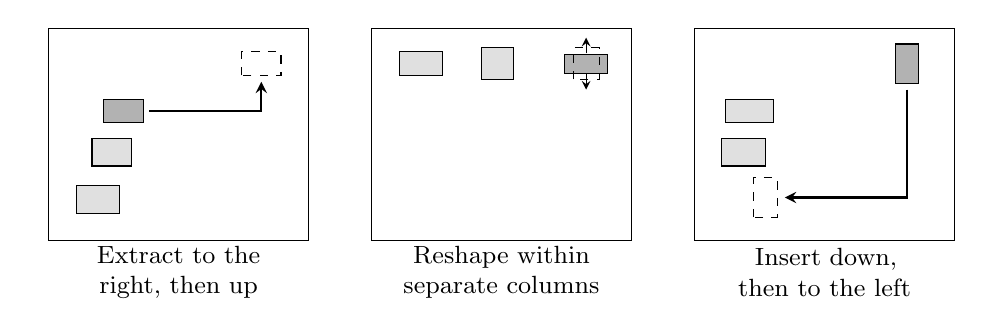
\begin{tikzpicture}[x=1cm,y=1cm,>=stealth,font=\small]
\begin{scope}
\draw (0,0) rectangle (3.3,2.7);
\draw[fill=black!12] (.35,.35) rectangle (.9,.7);
\draw[fill=black!12] (.55,.95) rectangle (1.05,1.3);
\draw[fill=black!30] (.7,1.5) rectangle (1.2,1.8);
\draw[dashed] (2.45,2.1) rectangle (2.95,2.4);
\draw[->,thick] (1.28,1.65)--(2.7,1.65)--(2.7,2.02);
\node[text width=3.6cm,align=center] at (1.65,-.4)
 {Extract to the right, then up};
\end{scope}
\begin{scope}[xshift=4.1cm]
\draw (0,0) rectangle (3.3,2.7);
\draw[fill=black!12] (.35,2.1) rectangle (.9,2.4);
\draw[fill=black!12] (1.4,2.05) rectangle (1.8,2.45);
\draw[fill=black!30] (2.45,2.13) rectangle (3,2.37);
\draw[dashed] (2.56,2.05) rectangle (2.89,2.45);
\draw[->] (2.725,2.38)--(2.725,2.58);
\draw[->] (2.725,2.12)--(2.725,1.92);
\node[text width=3.6cm,align=center] at (1.65,-.4)
 {Reshape within\\separate columns};
\end{scope}
\begin{scope}[xshift=8.2cm]
\draw (0,0) rectangle (3.3,2.7);
\draw[fill=black!12] (.35,.95) rectangle (.9,1.3);
\draw[fill=black!12] (.4,1.5) rectangle (1,1.8);
\draw[dashed] (.75,.3) rectangle (1.05,.8);
\draw[fill=black!30] (2.55,2) rectangle (2.85,2.5);
\draw[->,thick] (2.7,1.92)--(2.7,.55)--(1.15,.55);
\node[text width=3.6cm,align=center] at (1.65,-.4)
 {Insert down, then to the left};
\end{scope}
\end{tikzpicture}
\caption{The three routing stages, schematically.  Extraction is ordered
by decreasing source horizontal center; insertion is ordered by
increasing target horizontal center.  Those orders keep overlapping
vertical projections from becoming obstacles.  The source and target
families are separately disjoint; they need not be disjoint from one
another.}\label{fig:planar-routing}
\end{figure}

Figure~\ref{fig:planar-routing} summarizes the three routing stages.
We verify the required clearance for every pulse; this also treats
rectangles of unequal widths.  During horizontal extraction, consider
an unextracted rectangle whose vertical interval meets the active
one.  Since the source rectangles are disjoint, their horizontal
intervals are strictly separated.  The center ordering forces the
other interval to lie wholly to the left (equal centers would force
disjoint vertical intervals), so it cannot meet the
rightward swept box.  Previously parked rectangles lie near height
$3/4$, whereas sources lie below $1/2$.  The subsequent vertical
move is in a parking column, disjoint from both the source squares
near $X=1/4$ and the other parking columns.

During a scaling, each side length is between its initial and final
lengths, both at most $\lambda$.  Thus its entire motion lies in
$\boldsymbol\pi_r+[-\lambda/2,\lambda/2]^2$, separated from all
other parking boxes.  A vertical insertion again uses an empty parking
column and avoids the state squares.  During horizontal insertion,
parked rectangles are above the target heights.  Any previously
inserted target whose vertical interval meets the active target has
its horizontal interval wholly to the left, by disjointness and the
increasing-center order; it therefore does not meet the active
rectangle's leftward swept box, which stops at its own target.

All swept bounding boxes are contained in the open unit square.
They have rational endpoints, including the scaling bounding boxes,
and their distances to stationary boxes are positive.  Consequently
the cutoff recipe applies at every slot.  Induction through the
slots proves that every full source rectangle is moved according to
its assigned map, while all other tracked rectangles are held fixed
during that pulse.  The resulting period map is exactly
\eqref{eq:actual-branch} on every $D_r$.

The action holds on a positive neighborhood as well. For every slot,
include two kinds of clearance: the swept active rectangle's distance
from the complement of the region where its cutoff is one, and each
held rectangle's distance from the support of that cutoff. The cutoff
recipe gives effective positive lower bounds for both kinds. Minimize
these bounds over all slots and all tracked rectangles, obtaining $m>0$.
Let $M\ge1$ bound the operator norm of the linear part of every partial
affine product along every
branch, with the identity used during a held slot. Such a bound is
computed from the finitely many translations and reciprocal scalings.
Choose a rational radius $0<\rho<m/(2M)$. Induction through the slots
shows that a perturbation of norm less than $\rho$ stays in the active
one-plateau or the inactive zero-region, as appropriate. It therefore
follows the same affine formulas. All sources have been parked before
target insertion starts, so possible source--target overlaps introduce
no additional simultaneous obstacles. This proves neighborhood action
on whole rectangles, including their boundaries, with a radius computed
from the finite table and geometry rather than from its chosen execution.

The pulses vanish near all slot joints and phase endpoints; joining
them and repeating periodically gives a smooth $V$.  Every tracked
path has
\[
 1/4-\lambda\le X\le3/4+\lambda/2,
 \qquad 1/16\le Y\le3/4+\lambda/2,
\]
and hence lies in $J_*$.  For a branch whose source and target are
both nonterminal, \eqref{eq:state-height-bounds} and the parking height
give the stronger bound
\begin{equation}\label{eq:no-transient-halting}
 1/4-\lambda\le Y\le3/4+\lambda/2
 \quad\hbox{throughout the period}.
\end{equation}
Translations interpolate endpoint intervals, and the sole scaling
takes place at height $3/4$, so the bound includes all intermediate
times and all times when the rectangle is stationary.  Since
$\lambda<1/100$, its lower bound is greater than $3/16$.
The terminal square lies in $H$, at distance at least $1/32$ from
its boundary, because $\lambda<1/32$.

\begin{proof}[Completion of the proof of Theorem~\ref{thm:planar-processor}]
At integer phase times, induction using \eqref{eq:branch-table} proves
that the trajectory from $p$ has exactly the coordinates of the next
compiled configuration.  The radix code is interior to its appropriate
branch rectangle, including the left-symbol subrectangle for a left
move.  At ready checkpoints Lemma~\ref{lem:compiler} recovers the
original state and tape.  If absolute tape indices are desired, the
finite history block begins at absolute cell $2$: its tags and frontier
are visible in the two head-relative stacks, and so locate the head
relative to that cell.  Thus the correspondence encodes the computation,
not only its outcome.

If the machine halts, some integer phase time reaches the terminal
square.  If it does not, all consecutive states are nonterminal and
\eqref{eq:no-transient-halting} excludes $H$ at every time.  The smooth
field itself is defined everywhere for all phase times, so no issue
of continuation arises after a halting event.

All tables, rational rectangles, orders, clearances, and slots are
computed by finite procedures from the machine and its input.  The
only additional constants are computable numbers such as $\log B$.
The elementary cutoffs are computably smooth, not merely formal
piecewise descriptions: near a switching point the derivative estimates
in Lemma~\ref{lem:profiles} give effective smallness bounds, with the
fixed denominator lower bound $e^{-2}$.  Finite symbolic
differentiation and those bounds therefore produce effective uniform
bounds for every derivative of every pulse, including across all
joints and chart boundaries.  No test for exact equality of a real
argument with a switching point is needed to evaluate to a prescribed
accuracy.

Choose an effective $L\ge1$ bounding the operator norms of $D V$ and
$D^2 V$ uniformly.  The first variational equation gives
$\|D\Phi_s\|\le e^{Ls}$.  The second gives
\[
 \|D^2\Phi_s\|
 \le \int_0^s e^{L(s-r)}L e^{2Lr}\,dr
 =e^{2Ls}-e^{Ls}\le e^{2Ls}.
\]
For an arbitrary initial phase $s_0$ and length $s\ge0$, the inverse
of the transition map from $s_0$ to $s_0+s$ is the time-$s$ map of
\[
 \frac{dq}{dr}=-V(s_0+s-r,q),\qquad 0\le r\le s.
\]
This reversed nonautonomous field has the same global spatial derivative
bounds $L$. Its first and second variational equations therefore give
exactly the same bounds for the derivatives of the inverse map, on the
whole torus and for the compactly supported planar extension.  The difference of two lifted trajectories
satisfies the Lipschitz estimate $e^{Ls}$ as well.  In particular
every finite computational trajectory has an effective tube of
controlled radius: an initial perturbation of size
$\eta e^{-Ls}$ stays within $\eta$ up to time $s$.  This is a
finite-time estimate only, not a uniform robustness claim for an
infinite computation.
\end{proof}

\section{An autonomous spatial clock and a steady force}
\label{sec:lagrangian}

The planar phase can be supplied by the third spatial coordinate,
while retaining zero spatial mean.  This yields the following precise
form of forced Navier--Stokes universality.
Passing from a smooth return map to a three-dimensional flow is a
classical part of the generalized-shift construction
\cite[Section~6]{Moore1991}. Here we give the particular mean-zero
clock that equals unit speed on the entire tracked corridor.

\begin{proof}[Proof of Theorem~\ref{thm:main}]


Let $V$ be the field of Theorem~\ref{thm:planar-processor}.  Choose a smooth
cutoff $\chi_*(X,Y)$, equal to one near $J_*$ and compactly supported
in the open unit square, using the same rational-margin recipe as
above.  Extend its compactly supported products periodically.  Set
\begin{equation}\label{eq:autonomous-suspension}
 g(X,Y)=\partial_X\big(X\chi_*(X,Y)\big),\qquad
 W(X,Y,Z)=\big(V_1(Z,X,Y),V_2(Z,X,Y),g(X,Y)\big).
\end{equation}
This is a smooth periodic vector field.  Its divergence vanishes
because $V$ has zero planar divergence and $g$ is independent of $Z$.
Each component has zero spatial mean by its derivative representation.
Crucially, $g=1$ on a neighborhood of $J_*$; it need not be positive
on the whole torus.

For a planar computational segment starting at phase zero, the path
\[
 s\longmapsto (\Phi_s^V(X,Y),s\bmod1),\qquad 0\le s\le1,
\]
solves the autonomous $W$ equation, since the planar path stays in
$J_*$.  The smooth field has a unique global flow: periodicity gives
boundedness and a uniform spatial Lipschitz constant, so the standard
local ODE solution continues through every finite time.  Uniqueness
therefore identifies this displayed path with that flow.  Repeating
the argument period by period shows that the $W$ trajectory from $P$
encodes the compiled run at integer values of its path parameter $s$,
up to and including terminal entry if it occurs.  No absorbing motion
after terminal entry is required for the existential event.
The all-time exclusion and terminal inclusion in
Theorem~\ref{thm:planar-processor} prove the required reachability equivalence
for this autonomous flow.

To start from zero velocity, use the fixed ramp
\begin{equation}\label{eq:steady-ramp}
 \alpha(t)=\beta(2t-1),\qquad U(t,X,Y,Z)=\alpha(t)W(X,Y,Z),
\end{equation}
and prescribe
\begin{equation}\label{eq:steady-force}
 f(t)=\alpha'(t)W+\alpha(t)^2(W\cdot\nabla)W
          -\nu\alpha(t)\Delta W.
\end{equation}
Everything on the right is a previously constructed function, not an
unknown solution.  The ramp is zero near zero and equals one for
$t\ge1$.  Thus $f$ is eventually stationary and all its mixed
derivatives are bounded.  Its mean is zero: this holds for $W$ and
$\Delta W$, while
$\int_{\mathbb T^3}(W\cdot\nabla)W=0$ by periodicity and
$\nabla\cdot W=0$.  The residual identity gives the exact solution
$u=U$, $p=0$.  Lemma~\ref{lem:realization} supplies uniqueness in
the classical class on each finite time interval.
Since $U$ is uniformly bounded on a compact spatial domain, its
kinetic energy is uniformly bounded.

Material trajectories of $U$ are exactly those of $W$ with path
parameter
\[
 s(t)=\int_0^t\alpha(r)\,dr.
\]
This is continuous, finite at finite $t$, and has range $[0,\infty)$.
Indeed $\beta(u)+\beta(1-u)=1$, so $s(1)=1/4$ and
$s(t)=t-3/4$ for $t\ge1$.  Consequently every positive integer
computational phase $n$ occurs at physical time $n+3/4$.
The equivalence for $W$ transfers to the physical material flow,
including all intermediate times.

The force formula uses only the finite rule table, the finite input's
rational initial coordinates, and the finite routing construction.
Every branch is implemented in each phase cycle; the current fluid
position selects the next branch.  In particular evaluating the force
at a late physical time requires no evaluation of an equally long
machine run, and after time one the force has no time-dependent
instruction stream at all.  This proves effectiveness and the
absence of external replay.  Taking any fixed universal Turing
machine gives the asserted universal encoding.
\end{proof}

\begin{corollary}[Periodic forcing from time zero]\label{cor:periodic}
There is also an effective construction with zero initial velocity on
$\mathbb T^3$, a smooth mean-zero force of period one in time with
all mixed derivatives bounded, and the fixed particle event of
Theorem~\ref{thm:main}.
\end{corollary}

\begin{proof}
Take $U(t,X,Y,Z)=(V_1(t,X,Y),V_2(t,X,Y),0)$ directly from
Theorem~\ref{thm:planar-processor}.  Since $V$ vanishes near phase zero,
$U(0)=0$.  It is divergence free, mean zero, and periodic.  The
prescribed residual force
$f=\partial_tU+(U\cdot\nabla)U-\nu\Delta U$ has the same period,
mean, and bounded-derivative properties.  Lemma~\ref{lem:realization}
gives the unique global classical solution $U$, whose particle
trajectory from $(1/4,1/4,0)$ is exactly the planar processor trajectory
with third coordinate zero.  Theorem~\ref{thm:planar-processor} proves the
fixed-event equivalence.
\end{proof}

\begin{remark}[Solenoidal body forces]
Lemma~\ref{lem:projection} can replace the forces in
Theorem~\ref{thm:main} and Corollary~\ref{cor:periodic} by
effective mean-zero solenoidal forces, changing only the pressure.
It preserves the respective eventual stationarity or periodicity,
as well as all mixed-derivative bounds.  The velocity and its fixed
particle observable remain unchanged.
\end{remark}


\section{A slow clock with infinite accumulated time}\label{sec:profiles}
The autonomous spatial field also separates the geometric construction
from its physical rate of execution. Slowing it is legitimate only when
the accumulated path parameter still reaches every finite computational
time. The following statement makes that requirement explicit.

\begin{proposition}[Scalar clock]\label{prop:scalar-clock}
Let $W$ be the field \eqref{eq:autonomous-suspension}. Suppose
$a:[0,\infty)\to[0,\infty)$ is computably smooth, is zero near zero,
has an effective finite bound for $|a^{(h)}|$ for every integer
$h\ge0$ (including boundedness of $a$ itself), and
$\int_0^\infty a(t)\,dt=\infty$. Then
\[
 U_a(t,x)=a(t)W(x),\qquad
 F_a=a'W+a^2(W\cdot\nabla)W-\nu a\Delta W
\]
is a smooth mean-zero forcing construction with bounded mixed derivatives,
zero initial velocity and the same fixed-particle event as
Theorem~\ref{thm:main}. Its unique classical velocity is $U_a$.
For the specific choice
\begin{equation}\label{eq:slow-clock}
 a(t)=\frac{\beta(2t-1)}{1+t},
\end{equation}
every time order $h$ and spatial multi-index $\mu$ satisfy
\[
 \|\partial_t^h\partial_x^\mu U_a(t)\|_\infty+
 \|\partial_t^h\partial_x^\mu F_a(t)\|_\infty
 \le C_{h,\mu}(1+t)^{-1-h}.
\]
In particular all these spatial supremum norms belong to
$L^2(0,\infty)$, and the force tends uniformly to zero.
\end{proposition}
\begin{proof}
The residual formula is \eqref{eq:steady-force} with $\alpha=a$,
so Lemma~\ref{lem:realization} gives the solution and uniqueness.
The mean-zero and derivative assertions follow by differentiating the
three displayed coefficient functions. If $\gamma(s)$ is the trajectory
of $W$ from $P$, then $\gamma(s_a(t))$ solves the material equation,
where $s_a(t)=\int_0^t a(r)\,dr$. This clock is continuous,
nondecreasing, finite at each finite time and unbounded. The intermediate
value theorem gives $s_a([0,\infty))=[0,\infty)$, so the reachability
event is unchanged.

For \eqref{eq:slow-clock}, $a(t)=(1+t)^{-1}$ for $t\ge1$, and
\[
 s_a(t)=s_a(1)+\log\frac{1+t}{2}\qquad(t\ge1).
\]
Thus the clock is onto. The coefficients $a'$ and $a^2$ have time
derivatives of order $h$ bounded by a constant times $(1+t)^{-2-h}$,
whereas $a^{(h)}$ is bounded by a constant times $(1+t)^{-1-h}$.
All derivatives of the fixed spatial fields are bounded. These facts
give the claimed estimate for $t\ge1$; compactness gives an enlarged
constant on $[0,1]$. Squaring and integrating proves the $L^2$ claim.
\end{proof}

This slow profile and the eventually stationary profile are different
forces. An integrable nonnegative scalar clock would traverse only a
bounded amount of the same spatial trajectory and cannot replace the
onto-clock hypothesis. The present exact positional encoding and its
finite-time tube estimate also do not yield a uniform perturbation
tolerance for an unbounded computation.

\begin{corollary}[Undecidable fixed-particle reachability]
No algorithm decides the particle event for all finite force
descriptions constructed in Theorem~\ref{thm:main}.
\end{corollary}
\begin{proof}
Compose a proposed event algorithm with the terminating construction of
the force. The event equivalence would decide whether an arbitrary machine
halts on a finite input. It would therefore decide Turing's symbol-printing
problem \cite[Section~8]{Turing1936}: simulate a given machine and halt
exactly when its specified symbol is printed; if it stops without printing,
continue forever. Turing proves that no such decision procedure exists.
\end{proof}

\bibliographystyle{plain}
\bibliography{references}
\end{document}
